% Analítica Predictiva y Prescriptiva · TIC-60286 · Semana 1
% Predecir no es decidir
% Compilar: pdflatex week-01.tex (dos veces)
%
% Plan de los 90 minutos
%   0–10   El curso (láminas 2–5)
%  10–25   El paper: Google Flu Trends (láminas 6–9)
%  25–65   La aplicación: los cupos de Granada, la ficha, el encargo (láminas 10–21)
%  65–70   Puente: el task 1 (lámina 22)
%  70–90   Cierre: equipos y herramientas (lámina 23)
%
% Las figuras salen de datasets/week-01/_generar_latitud_cupos.R (semilla 29).
% Las cifras citadas están en datasets/week-01/cifras_week01.txt.
% ---------- identidad visual del curso (la paleta de styles.css) ----------

\documentclass{beamer}
\input{../../_beamer/preambulo_app.tex}
\semana{1}{Predecir no es decidir}

\begin{document}

%%=================================================
%% Primer slide
\begin{frame}
\titlepage
\end{frame}

%% ====================================================== 0. EL CURSO (0–10)
\begin{frame}{Qué es este curso y qué no}
\begin{columns}[T]
\begin{column}{0.5\textwidth}
\begin{exampleblock}{Es}
\begin{itemize}
  \item Un curso para gerentes que \textbf{dirigen} el análisis: preguntar, evidenciar, decidir.
  \item Nueve semanas sobre \textbf{una} decisión real de una empresa: cómo crecer con un presupuesto.
  \item Predictivo: árboles que predicen y un juez que los evalúa en pesos. Prescriptivo: costos, umbrales, escenarios, recomendación.
\end{itemize}
\end{exampleblock}
\end{column}
\begin{column}{0.5\textwidth}
\begin{alertblock}{No es}
\begin{itemize}
  \item Un curso de algoritmos ni de programación: no escribes código; el código corre en el navegador o lo escribe un agente que tú verificas.
  \item Un curso de automatización.
  \item Un curso donde la IA responde por ti: toda cifra sale de datos y de una ejecución, y tú la firmas.
\end{itemize}
\end{alertblock}
\end{column}
\end{columns}
\end{frame}

\begin{frame}{Las nueve semanas: una decisión, nueve piezas}
\small
\begin{tabular}{@{}c p{0.36\textwidth} p{0.5\textwidth}@{}}
\toprule
Sem. & Tema & Lo que el equipo produce \\
\midrule
1 & Predecir no es decidir; la pregunta & La ficha y la posición preliminar (hoy) \\
2 & Vigilar el entorno con datos alternativos & Tabla de señales con fuentes; dos incertidumbres críticas \\
3 & Explorar los datos con un agente & Tres hallazgos con cifra; la columna prohibida \\
4 & Juzgar modelos con dinero & Tabla del líder: consultora A, B o ninguna \\
5 & Árboles de clasificación & Reglas que se leen; umbral con costos \\
6 & Árboles de regresión & Ventas esperadas con su error \\
7 & Escenarios y decisión & Tabla de robustez; recomendación y disparadores \\
8 & Contar la historia & Memo de una página; validación con un experto \\
9 & Defensa ante la junta & La defensa; después, el memo individual \\
\bottomrule
\end{tabular}
\end{frame}

\begin{frame}{Cómo funciona cada semana}
\small
\begin{columns}[T]
\begin{column}{0.55\textwidth}
\begin{enumerate}
  \item \textbf{Antes:} la teoría, una página interactiva de 30 a 40 minutos. Mueves perillas, respondes preguntas, ejecutas sin escribir código.
  \item \textbf{La sesión:} un paper con una historia real (15 minutos), la aplicación al caso (45) y el cierre: 20 minutos para discutir el task que trajeron.
  \item \textbf{El task:} en equipo, una página, hacia el expediente. Se prepara para la sesión siguiente.
  \item \textbf{Práctica aparte} solo en las semanas de árboles (5 y 6): ahí hay que experimentar.
\end{enumerate}
\end{column}
\begin{column}{0.45\textwidth}
\begin{block}{La evaluación}
\begin{itemize}
  \item Tasks 2 a 8, en equipo: 45\,\% (cuentan los seis mejores).
  \item Defensa ante la junta: 35\,\% (expositor al azar).
  \item Memo individual de transferencia: 20\,\%.
\end{itemize}
Toda actividad admite IA con declaración de tres líneas.
\end{block}
\end{column}
\end{columns}
\end{frame}

\begin{frame}{Hoy}
\begin{itemize}\itemsep8pt
  \item Una predicción que le ganó al sistema oficial durante años, y lo que pasó después.
  \item Una zona de entregas, 56 días y una pregunta: si ya sabes cuántos pedidos van a llegar, ¿ya sabes cuántos cupos reservar?
  \item La ficha de la pregunta: siete campos que vas a llenar toda tu vida profesional.
  \item El encargo de la junta de Latitud.
\end{itemize}
\end{frame}

\seccion{El paper: Google Flu Trends}
%% ====================================================== 1. EL PAPER (10–25)
\begin{frame}{La primera gran victoria: Google Flu Trends}{Ginsberg et al. (2009), \emph{Nature}}
\begin{columns}[T]
\begin{column}{0.5\textwidth}
\textbf{Qué investigaron.} Si las búsquedas en Google permitían estimar la incidencia de gripe en Estados Unidos \emph{en tiempo real}.

\medskip
\textbf{El contexto.} La vigilancia oficial dependía de los reportes que los centros médicos envían a la CDC; agregarlos tomaba cerca de \textbf{10 días}. Demasiado para una epidemia.
\end{column}
\begin{column}{0.5\textwidth}
\textbf{Qué datos y cómo.}
\begin{itemize}
  \item Cientos de miles de millones de búsquedas de 2003 a 2008, por región, cruzadas con la curva oficial.
  \item Probaron cerca de \textbf{50 millones} de términos candidatos; el modelo final usa \textbf{45}.
  \item Sin teoría epidemiológica, sin encuestas, sin modelo estructural.
\end{itemize}
\end{column}
\end{columns}
\medskip
\importa{A Google le tomaba \textbf{un día} lo que a la CDC diez. ¿Convencidos?}
\end{frame}

\begin{frame}{La figura que convenció al mundo}{Ginsberg et al. (2009), figura 3}
\begin{center}
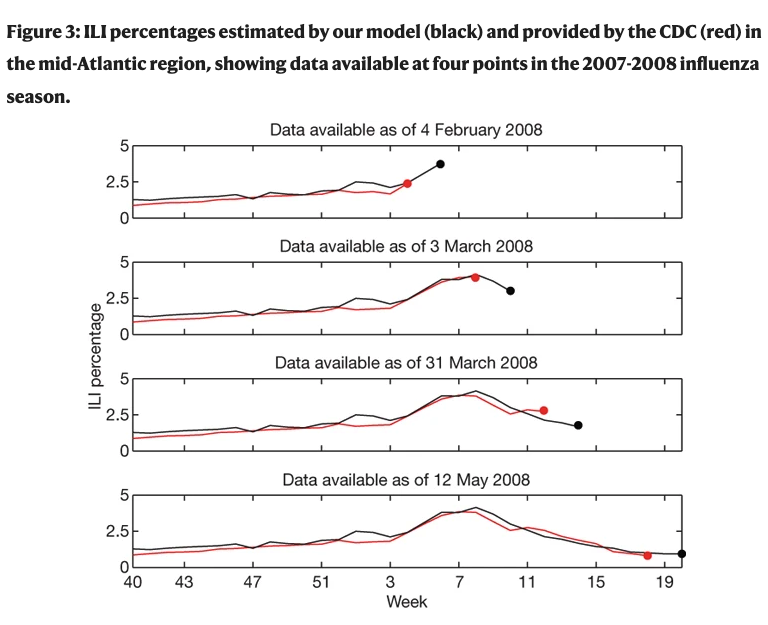
\includegraphics[height=0.47\textheight,trim=0 10 0 112,clip]{figures/ginsberg_fig3.png}
\end{center}
\vspace{-0.2cm}
{\scriptsize\color{gris} Región del Atlántico medio. Negro: porcentaje de consultas por síndrome gripal estimado por el modelo de Google con las búsquedas de esa misma semana. Rojo: el dato oficial de la CDC, que llega con una o dos semanas de rezago.}

\medskip
\textbf{Qué encontraron:} una curva construida con búsquedas sigue a la curva oficial semana a semana, y llega antes. ¿Qué puede salir mal?
\end{frame}

\begin{frame}{\ldots y su primera gran derrota}{Lazer, Kennedy, King y Vespignani (2014), \emph{Science}: ``The parable of Google Flu''}
\begin{itemize}\itemsep6pt
  \item En la temporada 2012--2013 Google Flu Trends predijo \textbf{más del doble} de los casos que ocurrieron.
  \item Sobreestimó la gripe en \textbf{100 de las 108 semanas} posteriores a agosto de 2011.
  \item ¿Qué salió mal?
  \begin{itemize}
    \item Con 50 millones de términos, muchos correlacionan con la gripe \textbf{por azar} (búsquedas de temporada, como las del baloncesto).
    \item El comportamiento de búsqueda \textbf{cambia}, y Google cambia su buscador: el modelo se entrenó en un mundo que dejó de existir.
    \item ``\emph{Big data hubris}'': creer que el tamaño de los datos sustituye la medición y la validación cuidadosas.
  \end{itemize}
\end{itemize}
\end{frame}

\begin{frame}{Por qué importa para quien decide}
\begin{block}{Tres lecciones que organizan este curso}
\begin{enumerate}\itemsep4pt
  \item Una predicción puede ser excelente durante años y \textbf{dejar de funcionar sin avisar}. Hay que vigilarla contra lo que pasa de verdad (semana 4).
  \item Lo que cuesta no es el error estadístico: es la \textbf{decisión que se tomó con él}. Un departamento de salud que compra vacunas o abre camas con una estimación doblada paga en pesos y en camas.
  \item Antes de celebrar la predicción, hay que preguntar \textbf{qué haría alguien distinto} con ella. Si la respuesta es ``nada'', no era una pregunta de decisión.
\end{enumerate}
\end{block}
\parada{el puente}{Si Latitud tuviera un Google Flu de los pedidos, sabría más o menos cuántos llegarán mañana. ¿Ya sabría cuántos cupos \textbf{reservar}?}
\end{frame}

\seccion{La aplicación: los cupos de Granada}
%% ====================================================== 2. LA APLICACIÓN (25–65)
\begin{frame}{Los cupos de Granada}
\begin{columns}[T]
\begin{column}{0.46\textwidth}
\small
\begin{itemize}\itemsep4pt
  \item Latitud, zona de Granada (Cali). Un operador logístico entrega los domicilios.
  \item Un pedido entregado deja \peso9.000 de margen. Un cupo reservado cuesta \peso2.000, se use o no; sin cupo, el pedido se cancela.
  \item 56 días, del 6 de enero al 2 de marzo de 2025: en promedio llegaron \textbf{115} pedidos al día; mínimo 78, máximo 161.
  \item Mariana, la coordinadora de operaciones, reserva el promedio.
\end{itemize}
\end{column}
\begin{column}{0.54\textwidth}
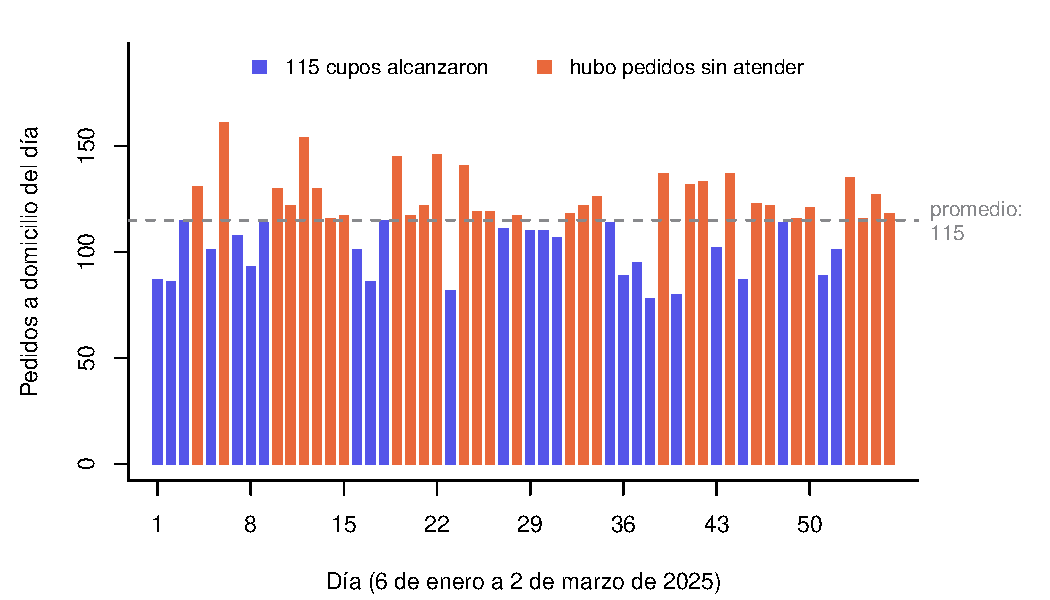
\includegraphics[width=\textwidth]{figures/demanda.pdf}
\end{column}
\end{columns}
\end{frame}

\begin{frame}{¿Cuántos cupos reservarías para mañana?}
\parada{encuesta}{Con lo que acabas de ver, ¿cuántos cupos reservas para mañana? \quad (a) 100 \quad (b) 115 \quad (c) 130 \quad (d) 145}
\medskip
Antes de hacer una sola cuenta. Después la repetimos.
\end{frame}

\begin{frame}{El pronóstico: 115}
\begin{columns}[T]
\begin{column}{0.5\textwidth}
\textbf{Lo que pasó con la regla del promedio, en los 56 días:}
\begin{itemize}
  \item en \textbf{31 días se agotaron los cupos} y hubo pedidos sin atender;
  \item en los otros 25 alcanzaron; contando todos los días, \textbf{7 cupos al día} se pagaron sin usarse;
  \item margen neto promedio: \textbf{\peso740.714 por día}.
\end{itemize}
\end{column}
\begin{column}{0.5\textwidth}
\importa{115 es un buen pronóstico: es el mejor número para describir un día cualquiera. La pregunta de hoy es si es una buena \textbf{decisión}.}
\end{column}
\end{columns}
\end{frame}

\begin{frame}{Dos errores, dos precios}
\begin{center}\small
\begin{tabular}{@{}l L{0.42\textwidth} L{0.36\textwidth}@{}}
\toprule
Error & Qué pasa & Cuánto cuesta cada unidad \\
\midrule
Sobrar & Se reserva un cupo que ningún pedido usa y se paga igual & \peso2.000 (la tarifa del cupo) \\
Faltar & Llega un pedido, no hay cupo y se cancela & \peso7.000 (el margen de 9.000 menos el cupo de 2.000) \\
\bottomrule
\end{tabular}
\end{center}
\medskip
\begin{itemize}
  \item Faltar cuesta \textbf{tres veces y media} lo que cuesta sobrar.
  \item La regla del promedio trata los dos errores como si pesaran lo mismo.
  \item \alert{Un pronóstico no sabe nada de esto.} Solo sabe de la demanda.
\end{itemize}
\end{frame}

\begin{frame}{A mano: tres días posibles}
Supongamos que mañana pueden llegar 90, 115 o 140 pedidos, cada caso con la misma probabilidad. En miles de pesos:
\[
\text{margen neto} = 9.000 \times \min(\text{cupos},\,\text{pedidos}) - 2.000 \times \text{cupos}
\]
\begin{center}\footnotesize
\begin{tabular}{@{}lcccc@{}}
\toprule
Cupos & Llegan 90 & Llegan 115 & Llegan 140 & \textbf{Promedio} \\
\midrule
115 & $810-230=580$ & $1.035-230=805$ & $1.035-230=805$ & \textbf{730} \\
125 & $810-250=560$ & $1.035-250=785$ & $1.125-250=875$ & \textbf{740} \\
140 & $810-280=530$ & $1.035-280=755$ & $1.260-280=980$ & \textbf{755} \\
\bottomrule
\end{tabular}
\end{center}
\medskip
Reservar 140 deja \peso25.000 más al día que reservar el promedio: más de \peso9 millones al año. Y en dos de cada tres días paga cupos sin usar.
\end{frame}

\begin{frame}{Un cupo más: ¿vale la pena?}
\small
\begin{columns}[T]
\begin{column}{0.53\textwidth}
El cupo adicional se \textbf{usa} si la demanda lo alcanza (gano 7.000) y se \textbf{paga sin usarse} si no (pierdo 2.000). Vale la pena mientras
\[
P(\text{se usa})\cdot 7.000 \;>\; P(\text{no se usa})\cdot 2.000,
\]
es decir, mientras la probabilidad de que la demanda \textbf{no} llegue hasta él sea menor que
\[
\frac{7.000}{7.000 + 2.000} = \frac{7}{9} \approx 0.78 .
\]
\end{column}
\begin{column}{0.45\textwidth}
\begin{block}{En los 56 días de Granada}
\begin{itemize}
  \item Llegaron 115 pedidos o menos el \textbf{45\,\%} de los días.
  \item Llegaron 130 o menos el \textbf{80\,\%} de los días.
  \item La reserva debe llegar hasta \textbf{130}.
\end{itemize}
\end{block}
El 0.78 es el \textbf{cuantil crítico}: la fracción de días que conviene cubrir.
\end{column}
\end{columns}
\end{frame}

\begin{frame}{La curva del margen neto, con los datos reales}
\begin{columns}[T]
\begin{column}{0.6\textwidth}
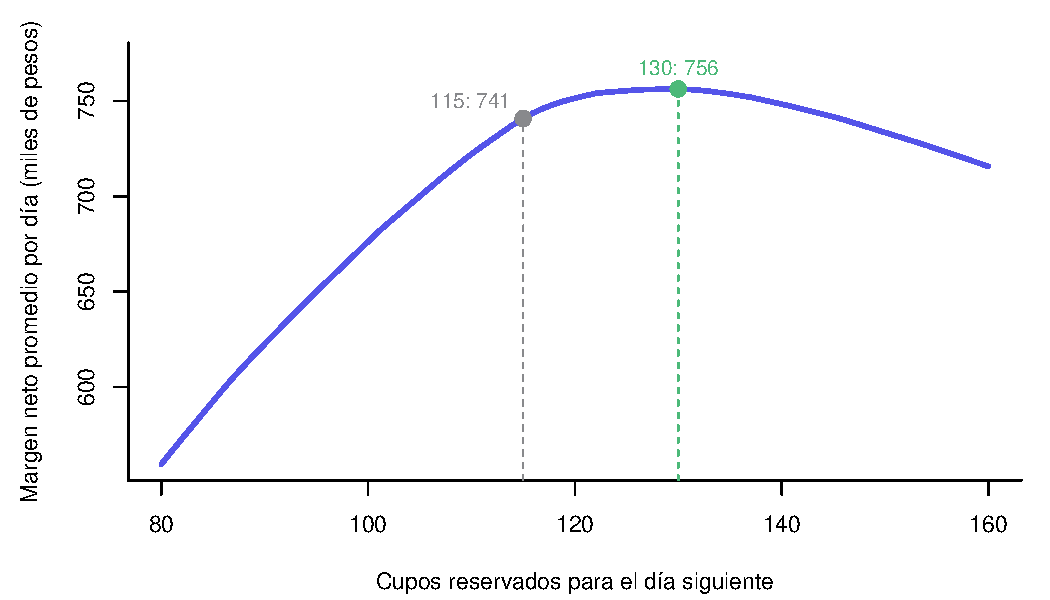
\includegraphics[width=0.96\textwidth]{figures/curva_margen.pdf}
\end{column}
\begin{column}{0.4\textwidth}
\small
\begin{itemize}\itemsep3pt
  \item Reservar 115: \peso740.714 por día.
  \item Reservar 130: \peso756.196 por día.
  \item La diferencia, \peso15.482 al día, son \textbf{\peso5.7 millones al año} en una sola zona de entrega.
  \item Días con pedidos sin atender: de 31 a 11. Cupos sin usar: de 7 a 17 por día.
\end{itemize}
\parada{segunda vez}{¿Y ahora cuántos reservarías?}
\end{column}
\end{columns}
\end{frame}

\begin{frame}{Lo que importa}
\importa{%
\begin{enumerate}\itemsep5pt
  \item \textbf{Predecir no es decidir.} El pronóstico (115) no cambió en ningún momento; cambió la decisión (130), porque miramos lo que cuesta cada error.
  \item \textbf{La asimetría manda.} Cuando faltar cuesta más que sobrar, se decide por encima del pronóstico; cuando cuestan parecido, el promedio es casi la mejor decisión.
  \item \textbf{El mejor modelo del mundo no reemplaza esta cuenta.} Google Flu habría predicho la gripe; alguien tenía que decidir cuántas vacunas comprar.
\end{enumerate}}
\end{frame}

\begin{frame}{La ficha de la pregunta}{El caso de una empresa de telecomunicaciones}
\footnotesize
Una telco pierde el 25\,\% de sus clientes al año. Cada cliente perdido cuesta \peso500; un incentivo de retención cuesta \peso100 y evita 6 de cada 10 abandonos. Un modelo encuentra a 75 de cada 100 clientes que se van y acierta en 60 de cada 100 a los que señala.
\smallskip
\begin{tabular}{@{}p{0.3\textwidth}p{0.66\textwidth}@{}}
\toprule
1. La decisión & A quiénes enviarles el incentivo este mes \\
2. Las alternativas & La lista del modelo; a todos; a nadie \\
3. Quién decide y cuándo & El gerente de retención, cada mes \\
4. El horizonte & El trimestre \\
5. El criterio y su unidad & Pesos retenidos menos incentivos pagados \\
6. El costo de cada error & Enviar a quien no se iba: \peso100. No enviar a quien se iba: \peso500 $\times$ 0.6 $=$ \peso300 esperados \\
7. El dato que cambiaría la decisión & La efectividad real del incentivo \\
\bottomrule
\end{tabular}
\end{frame}

\begin{frame}{¿Y si el incentivo cuesta \peso2.000?}
\parada{encuesta}{Con el incentivo a \peso2.000, ¿a quién le envías? \quad (a) a los mismos \quad (b) solo a los más seguros \quad (c) a nadie}
\small
\begin{itemize}\itemsep3pt
  \item Enviar a quien no se iba cuesta ahora \peso2.000; no enviar a quien se iba sigue costando \peso300. La lista se encoge hasta los clientes de los que el modelo está casi seguro.
  \item El modelo no cambió. Cambió la métrica que importa: de ``¿a cuántos encuentro?'' a ``¿en cuántos acierto?''. \textbf{La métrica sale del negocio.} Con números, en la semana 4.
\end{itemize}
\begin{alertblock}{Error sembrado}
Una ficha que recibí dice en el campo 1: ``\emph{Aumentar la participación de mercado del Club}''. ¿Qué está mal?
\end{alertblock}
\end{frame}

\begin{frame}{El encargo de la junta de Latitud}
\begin{columns}[T]
\begin{column}{0.45\textwidth}
\textbf{Latitud S.A.S.} 46 tiendas de conveniencia en Cali, Bogotá y Medellín, un centro de distribución en Yumbo y el Club Latitud (cerca de 4.000 suscriptores).

\medskip
El flujo de caja de 2026 deja \textbf{\peso1.000 millones} para crecer.

\medskip
La junta no ha dicho cómo juzgará una buena recomendación. Proponerlo es parte del trabajo.
\end{column}
\begin{column}{0.55\textwidth}
\footnotesize
\begin{tabular}{@{}c L{0.5\linewidth} L{0.32\linewidth}@{}}
\toprule
 & Alternativa & Costo aprox. \\
\midrule
A & Entrar a Barranquilla: la primera tienda (tres locales candidatos) & \peso700 millones \\
B & Acelerar el Club, por tramos & \peso150 millones por tramo, hasta 3 \\
C & Un piloto: un punto de formato reducido en Barranquilla, seis meses & \peso120 millones \\
D & Esperar un año: mejoras menores y caja & --- \\
\bottomrule
\end{tabular}
\end{column}
\end{columns}
\end{frame}

\begin{frame}{El expediente: nueve piezas, una defensa}
\begin{columns}[T]
\begin{column}{0.55\textwidth}
\begin{enumerate}\small
  \item La ficha de la pregunta y la posición preliminar (sellada)
  \item La vigilancia del entorno y las dos incertidumbres críticas
  \item Los hallazgos de los datos y la columna prohibida
  \item El juicio de los modelos comprados
  \item El árbol de clasificación: reglas y umbral
  \item El árbol de regresión: ventas esperadas con error
  \item Los escenarios y la tabla de robustez
  \item El memo y la validación con un experto
  \item La defensa y el memo individual
\end{enumerate}
\end{column}
\begin{column}{0.45\textwidth}
\importa{Se califica el expediente, no el desenlace. Una recomendación de esperar, bien sustentada, vale lo mismo que una de abrir.}
\end{column}
\end{columns}
\end{frame}

\seccion{El task y el cierre}
%% ====================================================== 3. PUENTE (65–70)
\begin{frame}{Task 1: la ficha de Latitud}
\begin{columns}[T]
\begin{column}{0.55\textwidth}
\textbf{Qué se entrega} (una página, en equipo, antes de la sesión 2):
\begin{itemize}
  \item las dos variantes de los cupos: el operador devuelve \peso1.000 por cupo no usado; la tarifa del cupo sube a \peso4.000;
  \item la ficha de la decisión de la junta, con [por confirmar] donde falte el dato;
  \item la posición preliminar, en el cuestionario de Canvas: qué harían hoy, por qué, y qué supuesto los haría cambiar. Se sella hasta la semana 9.
\end{itemize}
\end{column}
\begin{column}{0.45\textwidth}
\begin{exampleblock}{En el cierre de la sesión 2}
Dos equipos al azar muestran su ficha, dos minutos cada uno. La pregunta: \textbf{¿qué dato cambiaría su decisión y cuánto costaría conseguirlo?}
\end{exampleblock}
\end{column}
\end{columns}
\end{frame}

%% ====================================================== 4. CIERRE (70–90)
\begin{frame}{Cierre: equipos y herramientas}
\begin{enumerate}\itemsep8pt
  \item \textbf{Equipos de tres} (5 minutos). Escriban los nombres en el chat; son los equipos de todo el curso.
  \item \textbf{La teoría en el navegador} (5 minutos). Abran la página de la semana 1, muevan la perilla hasta 130 y luego cambien la tarifa del cupo a \peso4.000. ¿Hacia dónde se movió la mejor cantidad?
  \item \textbf{La decisión en una línea} (5 minutos). Cada equipo escribe en el chat el campo 1 de su ficha de Latitud, empezando por un verbo. Leemos cinco.
  \item \textbf{Dudas} (5 minutos): Canvas, el expediente, la entrega del task.
\end{enumerate}
\end{frame}

\begin{frame}{Referencias}
\small
\begin{itemize}\itemsep5pt
  \item Ginsberg, J., Mohebbi, M. H., Patel, R. S., Brammer, L., Smolinski, M. S. y Brilliant, L. (2009). Detecting influenza epidemics using search engine query data. \emph{Nature}, 457, 1012--1014.
  \item Lazer, D., Kennedy, R., King, G. y Vespignani, A. (2014). The parable of Google Flu: traps in big data analysis. \emph{Science}, 343(6176), 1203--1205.
  \item Sosa Escudero, W. (2019). \emph{Big data: breve manual para conocer la ciencia de datos que ya invadió nuestras vidas}. Siglo XXI. Capítulo 1.
\end{itemize}
\end{frame}

\end{document}
